\chapter{Konzepte von Predictive Analytics}
\label{part:Konzepte_PA}

\section{Begriffsdefinition}

Das primäre Ziel von \emph{\gls{glos:Predictive_Analytics}} ist das Treffen von
Vorhersagen.
Hierbei sind nicht nur Prognosen für die Zukunft gemeint, sondern
auch Einschätzungen und Beurteilungen unklarer Situationen, bei denen die für
die Entscheidungsfindung wichtigen Daten fehlen (vgl. \cite{Dinov}, S.~9~f.).
Hier sind einige Anwendungsbeispiele, die verdeutlichen, wie \emph{predictive
analytics} eingesetzt werden kann (vgl. \cite{Schmitz}):
\begin{description}
\item[Betrugserkennung (\emph{fraud detection}):] \hfill \\
Geschäftsvorgänge werden automatisch analysiert, in der Hoffnung, dass
Unregelmäßigkeiten vom System erkannt werden. Verdächtige Vorgänge können dann
zum Beispiel einer manuellen Prüfung unterzogen werden.


\item[Vorhersage von Wartungszeitpunkten (\emph{predictive
  maintenance}):] \hfill \\
Automatische Systeme schätzen die Ausfallwahrscheinlichkeit von Maschinen ein
und bestimmen den Zeitpunkt für die nächste Inspektion.
\item[Verringerung von Ausschuss (\emph{predictive quality}):]
Mit Hilfe von Sensordaten werden fehlerhafte Produkte im Produktionsprozess
erkannt und aussortiert.
\item[Erkennung von Kundenunzufriedenheit (\emph{churn management}):]
Muster in Daten, die auf Unzufriedenheit von Kunden deuten, automatisch erkennen
und rechtzeitig Gegenmaßnahmen versuchen.
\item[Verbesserung der Zahlungsmoral:]
Mit Hilfe von Vorhersagen die Randbedingungen verbessern, sodass Kunden
schneller Rechnungen begleichen.
\item[Bessere Kontrolle von Personalfluktuationen:]
Mitarbeiter, die bald einen Arbeitsplatzwechsel vollziehen könnten, mit Hilfe
von Vorhersagemodellen erkennen, um rechtzeitig darauf reagieren zu können.
\end{description}
\begin{figure}%[!hbt]
\centering
\caption{Erstellung von Vorhersagemodellen.}
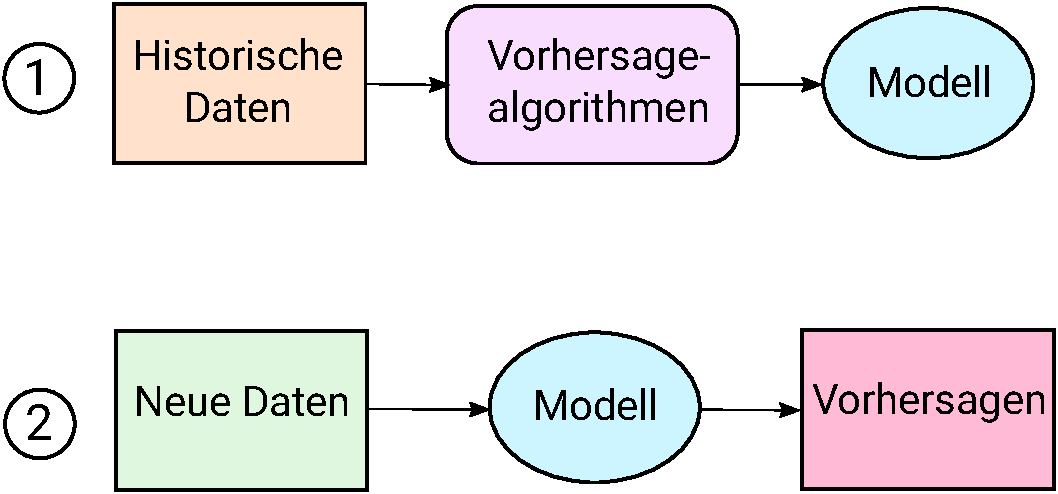
\includegraphics[scale=0.8]{Grafiken/PA_Ink.pdf} 
\label{pic:PA}
\end{figure}
Abbildung~\ref{pic:PA} veranschaulicht den allgemeinen Prozess zur Generierung
von Vorhersagemodellen\footnote{
Basierend auf dem Original aus \cite{Parthasarathy}.
}.
Zum Erstellen der Vorhersagen werden historische Daten benötigt. Diese Daten
werden von Algorithmen genutzt, um Modelle zu bauen. Die Vorhesagemodelle
akzeptieren neue Daten als Eingabe und liefern dazu eine Vorhesage der
gewünschten Eigenschaften. So könnte eine Versicherung beispielsweise
Vorhersagemodelle zur Betrugserkennung implementieren. Die historischen Daten
könnten in diesem Fall Forderungen von Kunden an die Versicherung aus der
Vergangenheit sein. Das Vorhesagemodell würde dann eine neue Forderung an die
Versicherung als Eingabe nehmen und könnte als Ausgabe eine Zahl zwischen 0 und
1 liefern. Dieser vorhergesagte Wert kann dann als Wahrscheinlichkeit
interpretiert werden, dass es sich bei der neuen Forderung um einen Betrugsfall
handelt. 

\section{Begriffsabgrenzung}

Unter \emph{data mining} versteht man das Nutzen von statistischen Methoden zur
Analyse großer Datenmengen mit dem Ziel, neue Erkenntnisse zum untersuchten 
Thema oder Objekt zu erlangen\footnote{
Der Begriff \emph{data mining} ist also nicht wörtlich zu verstehen. Gemeint ist
nicht die Gewinnung von Daten, sondern die Gewinnung von Erkenntnissen aus den
Daten.
}
(vgl. \cite{McCarthy}, S.~6). Es bestehen große Schnittmengen mit
\emph{predictive analytics}, insbesondere im Hinblick auf die Nutzung der
gleichen Methoden und Werkzeuge. Allerdings steht bei \emph{data mining} nicht
explizit die Erstellung von Vorhersagen im Vordergrund.

\emph{Data science} kann als interdisziplinäres Feld verstanden werden, das mit
großen und komplexen Datenbeständen arbeitet. Das Ziel von \emph{data science}
ist die Entwicklung von Algorithmen und Werkzeugen, die in der Lage sind, diese
Datenbestände zu nutzen, um Systeme zur Entscheidungsunterstützung zu
implementieren (\emph{semiautomated decision support systems}) (vgl.
\cite{Dinov}, S.~9).  Im Gegensatz zu \emph{predictive analytics} steht bei 
\emph{data science} eher die Entwicklung von Algorithmen im Vordergrund. 
Bei \emph{predictive analytics} hingegen steht die Anwendung dieser Methoden im 
Fokus.

\emph{Business analytics} wird als Oberbegriff für Prozesse definiert, die
Analysemodelle im geschäftlichen Kontext erstellen . \emph{Predictive analytics}
und \emph{data mining} werden dann als Bestandteil von \emph{business analytics}
gesehen. (vgl. \cite{McCarthy}, S.~6))

\emph{Business intelligence} ist ein zu \emph{business analytics} ähnlicher
Begriff und steht allgemein für Anwendungen und Techniken, die im
Geschäftsumfeld zur Entscheidungsunterstützung und zur Generierung von
Einsichten genutzt werden\footnote{
Manche Autoren betrachten den Begriff \emph{intelligence} als Anspielung auf die
gängige, englische Bezeichung für Aufklärungs- und Nachrichtendienste, wie
beispielsweise die CIA.
} (vgl. \cite{Gluchowski}, S.~89-90). Damit kann \emph{predictive analytics},
ähnlich wie bei \emph{business analytics}, als ein Bestandteil von 
\emph{business intelligence} eingeordnet werden (vgl. \cite{Gluchowski}, S.~92). 

Ein in diesem Zusammenhang weniger verbreiteter Begriff ist \emph{forecasting},
die Erstellung von Prognosen durch menschliche Beobachter. Im nächsten Abschnitt
wird diese Form von Vorhersagen genauer beschrieben und anschließend mit
\emph{predictive analytics} verglichen.  

\section{Probleme menschlicher Urteile}

Die meisten Urteile und Prognosen werden von Menschen gefällt, ohne statistische
Modelle und Vorhersagealgorithmen zu nutzen. Grundsätzlich fällt jeder Mensch
Urteile, macht Vorhersagen und nutzt diese um Entscheidungen zu treffen. Aus
diesem Grund ist ein gutes Urteilsvermögen eine Eigenschaft, die eigentlich
universell gebraucht wird. Für die großen gesellschaftlichen Entscheidungen
versorgen Experten Wirtschaft, Politik und Öffentlichkeit mit Prognosen und
Einschätzungen. Dabei ist es üblich routinemäßig Expertenmeinungen einzuholen,
unüblich ist es allerdings, systematisch die Qualität dieser Urteile zu
überprüfen (vgl. \cite{Tetlock}, S.~1). Aus diesem Grund hat der Psychologe
Philip Tetlock sich zur Aufgabe gemacht, \glqq{gutes} Urteilsvermögen\grqq
formal fassbar zu machen (vgl. \cite{Tetlock}, S.~3). Nach Tetlock sollte gutes
Urteilsvermögen anhand zweier Kriterien gemessen werden (vgl. \cite{Tetlock},
S.~7):
\begin{description}
\item[(1) Richtigkeit der Vorhersagen (\emph{get it right}):]
\label{misc:Emp_Korr}
Empirische Korrespondenztests sollen genutzt werden, um zu überprüfen, wie gut
die Meinungen und Vorhersagen von Experten mit der Wirklichkeit übereinstimmen.
\item[(2) Logische Konsistenz des Denkmodells (\emph{think the right way}):]
Die Gedanken von Experten sollten logisch konsistent sein. Genauer ausgedrückt
bedeutet dies, dass die Denkmodelle nicht die Gesetze der Logik und der
Statistik missachten sollten. Zudem sollte eine Person mit einem guten
Urteilsvermögen ihre Glaubenssätze an neue Erkenntnisse anpassen können.
\end{description}
Dabei sollte die experimentelle Psychologie die notwendigen Fakten und
Einsichten liefern (vgl. \cite{Tetlock}, S.~8).

\subsection{Tetlocks Forecasting Exercises}

Für die empirischen Korresponenztests führten Tetlock und sein Team eine Reihe
von \emph{forecasting exercises} mit Experten durch. Diese Expertenbefragungen
wurden bereits in Teil~\ref{part:Schw_Vorhersagen} thematisiert und sollen nun
detaillierter erläutert werden. \\ \\
Insgesamt wurden die Urteile von 284 Experten analysiert. Diese hatten im
Durchschnitt 12 Jahre Berufserfahrung und die Hälfte (52~\%) besaß einen
Doktortitel. Etwa 61~\% der Teilnehmer wurden mindestens einmal von den Medien
interviewt und 21~\% mehr als zehnmal. Etwa 80~\% der Experten waren mindestens
einmal als Berater für internationale politische oder wirtschaftliche
Angelegenheiten tätig. (vgl. \cite{Tetlock}, S.~239-240)\\ \\
Die Befragten sollten Prognosen erstellen, indem sie auf Fragen zu zukünftigen
Entwicklungen in Politik und Wirtschaft antworteten. Dabei handelte es sich um
feste Fragestellungen, die von den Forschern zuvor ausgewählt wurden. Zu den in
den Fragen formulierten Szenarien sollten die Befragten subjektive
Wahrscheinlichkeiten\footnote{
Eine subjektive Wahrscheinlichkeit wird als Grad des Vertrauens einer Person in
den Eintritt eines Ereignisses interpretiert (vgl. \cite{Eisenfuehr}, S.~152).}
angeben. (vgl. \cite{Tetlock}, S.~245)\\ \\
Die Sammlung der Expertenprognosen begann 1987 und erstreckte sich über mehr als
zehn Jahre. Dabei wurden Fragen über die zukünftige Entwicklung von etwa 60
Nationen gestellt. (vgl. \cite{Tetlock}, S.~242)\\ \\
Weiterhin wurden die Fragen in folgende Themenbereiche untergliedert
(vgl. \cite{Tetlock}, S.~246-248):
\begin{description}
\item[(a)] Kontinuität politischer Führung
\item[(b)] Innen- und Wirtschaftspolitik
\item[(c)] Nationale Sicherheit und Verteidigungspolitik
\item[(d)] Zusätzliche Spezialthemen
\end{description}
Insgesamt wurden 82 361 subjektive Wahrscheinlichkeiten eingeholt, die als
Antwort auf circa 27 450 Fragen gegeben wurden. (vgl. \cite{Tetlock}, S.~246)

\subsection{Der Probability Score als Maß der Genauigkeit von Vorhersagen}

Die Fragen der \emph{forecasting exercises} wurden so formuliert, dass bei allen
nach einer gewissen Zeitspanne festgestellt werden konnte, ob und welches der
möglichen Szenarien\footnote{
Die möglichen Szenarien müssen dabei logisch vollständig sein und sich
gegenseitig ausschließen (\emph{logically exhaustive and mutually exclusive};
vgl. \cite{Tetlock}, S.~245).
} tatsächlich eingetreten ist. Um dann die, auf Seite~\pageref{misc:Emp_Korr}
erwähnte, Richtigkeit der Vorhersagen zu überprüfen, müssen die subjektiven
Wahrscheinlichkeiten mit der eingetretenen Wirklichkeit verglichen werden. \\ \\
Das Werkzeug zur Durchführung dieses Vergleichs und zur Bewertung der
Genauigkeit der erstellten Prognosen ist der \emph{probability score}\footnote{
  Auch \emph{Brier score} genannt (siehe \xcom)
} (vgl. \cite{Tetlock}, S.~46). Dabei werden die subjektiven
Wahrscheinlichkeiten (die Vorhersagen) mit den tatsächlich eingetretenen
Ereignissen (der Wirklichkeit) verrechnet\footnote{
  Es wird 0 eingesetzt, falls ein Szenario nicht eingetreten ist und 1 falls es
  eingetreten ist (vgl. \cite{Tetlock}, S.~46-47).
}. Das Ergebnis ist eine Zahl zwischen 0 und 1, wobei 0 die beste und 1 die
schlechteste Wertung darstellt. Wenn ein Prognostiker jedes Ereignis, das
schließlich eintritt, als unmöglich eingestuft hat und jedes Ereignis, welches
ausbleibt, als sicher, dann endet er beim schlechtesten \emph{probability
score} von 1. Die beste Wertung von 0 kann hingegen nur erreicht werden, indem
man, zumindest was die gestellten Fragen betrifft, hellseherische Fähigkeiten
beweist und jedes eingetretene Ereignis mit einer subjektiven Wahrscheinlichkeit
von 1 bewertet und jedem ausgebliebenen Ereignis eine 0 zugewiesen hat (vgl.
\cite{Tetlock}, S.~47). \\ \\
Zudem lässt sich der \emph{probability score} in zwei Komponenten zerlegen, die
von den Fähigkeiten des Prognostikers abhängen: Kalibrierung
(\emph{calibration}) und Diskriminierung (\emph{discrimination})\footnote{
  Die Bedeutung dieser beiden Komponenten wurde auch im einleitenden
  Teil~\ref{part:Schw_Vorhersagen} erläutert.
} (vgl. \cite{Tetlock}, S.~47). \\ \\
Die Kalibrierung misst wie gut ein Prognostiker
Ereignisse in Wahrscheinlichkeitskategorien einordnen kann\footnote{
  10~\% der Ereignisse aus der 0.1 Kategorie treten ein, 20~\% der Ereignisse
  aus der 0.2 Kategorie usw. 
}. Der Wertebereich der Kalibrierung liegt zwischen 0 und 1, wobei 0 den besten
und 1 den schlechtesten Wert darstellt (vgl. \cite{Tetlock}, S.~275). \\ \\
Die Diskriminierung misst wie gut sich die subjektiven Wahrscheinlichkeiten des 
Prognostikers von der relativen Häufigkeit (\emph{base-rate}) aller betrachteten
Ereignisse abheben. Der Wertebereich der Diskriminierung reicht von 0 bis zu
einem Wert, der die Unsicherheit der Umgebung, für die die Prognosen erstellt
werden, widerspiegelt (vgl. \cite{Tetlock}, S.~278). Im Falle der
Diskriminierung ist 0 der schlechteste Wert. Im besten Fall ist der Wert der
Diskriminierung gleich dem Wert der Unsicherheit. \\ \\
Die Kernidee bei der Anwendung des \emph{probability score} ist das Nutzen
des Gesetzes der großen Zahlen (\emph{law of large numbers})
(vgl. \cite{Tetlock}, S.~12-13). Einzelne Urteile mit subjektiven
Wahrscheinlichkeiten, die nicht 0 oder 1 sind, können nicht widerlegt werden,
da seltene Ereignisse eintreten können und häufige Ereignisse ausbleiben können.
Betrachtet man hingegen eine große Zahl an Vorhersagen, dann kann mit Hilfe
des \emph{probability score} die Genauigkeit des Prognostiker aus der Gesamtheit
seiner Vorhersagen eingeschätzt werden. \\ \\
Der Anhang~\xcom liefert die Formeln für den \emph{probability score}, wobei
dessen Berechnung zusätzlich anhand von Beispielen erläutert wird. \\ \\

\subsection{Detaillierte Ergebnisse der Forecasting Exercises}

Die Analyse der Ergebnisse der \emph{forecasting exercises} konnte Aufschluss
darüber geben, welche Attribute der Teilnehmer einen Einfluss auf die
Genauigkeit ihrer Vorhersagen haben und welche nicht. \\ \\
Zu den Attributen, die keinen Einfluss auf die Fähigkeiten der Experten haben,
gehören überraschenderweise (vgl. \cite{Tetlock}, S.~68):
\begin{itemize}
\item der Bildungsgrad (Doktortitel oder kein Doktortitel)
\item das Fachgebiet
\item die Erfahrung
\item der Zugang zu geheimen Informationen
\end{itemize}
Zudem hat Medienberühmtheit einen starken negativen Effekt auf die Fähigkeiten
der Prognostiker (vgl. \cite{Tetlock}, S.~68). \\ \\
Ein entscheidender Faktor, der gute von schlechte Prognostikern unterscheidet,
ist nicht ihr Weltbild, sondern ihre Art zu Denken (\emph{cognitive style})
(vgl. \cite{Tetlock}, S.~72 und S.~75). Tetlock unterteilt die Experten in
Abhängigkeit von ihrer Art zu Denken in Füchse (\emph{foxes}) und Igel
(\emph{hedgehogs})\footnote{
In Anlehnung an das Essay \emph{The Hedgehog and the Fox} des Philosophen Isaiah
Berlin.
}. Genauer ausgedrückt, ist das wichtigste Maß für den \emph{cognitive style}
eines Experten ein Wert auf einer kontinuierlichen Skala (vgl. \cite{Tetlock},
S.~87). An einem Ende der Skala befinden sich die \emph{foxes}, an dem anderen
die \emph{hedgehogs}. Dazwischen befinden sich die hybriden Ausprägungen
\emph{fox-hog} (eher \emph{fox} als \emph{hedgehog}) und \emph{hedge-fox} (eher
\emph{hedgehog} als \emph{fox}). Bestimmt wird der Wert als Ergebnis eines
Fragebogens (siehe \cite{Tetlock}, S.~241). Dabei ist der Punkt, der am
stärksten in die Gewichtung einfließt, die Frage nach der Selbstidentifikation
(vgl. \cite{Tetlock}, S.~74 Tabelle~3.3)\footnote{
Hierbei werden Gewichtungen angegeben, mit denen die einzelnen Fragen in
die Bewertung einfließen. Je höher der Betrag des Gewichts, desto stärkeren
Einfluss hat die Frage auf das Ergebnis. Das Vorzeichen des Gewichts gibt an,
in welche Richtung die jeweilige Frage das Ergebnis verschiebt. Ein negatives
Vorzeichen verschiebt den Wert auf der Skala in \emph{hedgehog} Richtung, ein
positives Vorzeichen hingegen in \emph{fox} Richtung.   
}. Diese Frage lautet übersetzt (siehe \cite{Tetlock}, S.~241):
\begin{quotation}
%\begin{spacing}{1.2}
Isaiah Berlin unterteilte Intellektuelle in Igel und Füchse. Der Igel kennt eine
große Sache und versucht so viel wie möglich innerhalb dieses konzeptionellen
Rahmens zu erklären, wohingegen der Fuchs viele kleine Dinge weiß und damit
zufrieden ist, von Fall zu Fall andere improvisierte Erklärungen zu
finden. Ich positioniere mich zum Igel- oder Fuchsende dieser Skala.
% Isaiah Berlin classified intellectuals as hedgehogs or
% foxes. The hedgehog knows one big thing and tries to explain as much as
% possible within that conceptual framework, whereas the fox knows
% many small things and is content to improvise explanations on a case-
% by-case basis. I place myself toward the hedgehog or fox end of this
% scale
%\end{spacing}
\end{quotation}
Abbildung~\ref{pic:Hedgehog_Fox} erläutert die Skala des \emph{cognitive style}.
\\ \\
\begin{figure}%[!hbt]
\centering
\caption{Skala des \emph{cognitive style}%, mit den Charakterisierungen
%  \emph{Fox} und \emph{Hedgehog} als Gegenpole}
}
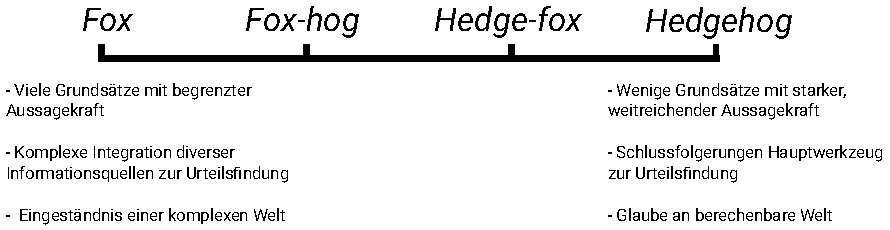
\includegraphics[scale=1]{Grafiken/Hedgehog_Fox.pdf} 
\label{pic:Hedgehog_Fox}
\end{figure}
\emph{Hedgehogs} haben einige wenige Glaubenssätze, die sie nutzen um
Erklärungen für die unterschiedlichsten Dinge abzuleiten (vgl. \cite{Tetlock},
S.~73). Sie bemühen sich, Fakten in Einklang mit ihren präferierten Grundsätzen
zu bringen und fällen ihre Urteile, indem sie Schlussfolgerungen aus einer
kleinen Menge an Überzeugungen ziehen. Zudem tendieren \emph{hedgehogs}
zu intellektuellem \glqq{Geiz}\grqq (\emph{parsimony}) (vgl.\cite{Tetlock}, 
S.~20). Dies bedeutet, dass sie nur ungerne neue Grundsätze
aufstellen und stattdessen versuchen, mit ihren wenigen, schon vorhandenen
Glaubenssätzen weitreichende Erklärungen für eine große Bandbreite an Phänomenen
zu erhalten. Zudem zeichnen sich \emph{hedgehogs} durch eine starke
Selbstsicherheit in Bezug auf die Genauigkeit ihrer Prognosen und Urteile aus
(vgl. \cite{Tetlock}, S.~73). \\ \\
\emph{Foxes} hingegen sind skeptisch bezüglich starker Glaubenssätze, die alles
umspannende Erklärungen liefern sollen. Stattdessen vertrauen sie auf viele
Grundsätze mit begrenzter Aussagekraft (\emph{tricks of their trade}) (vgl.
\cite{Tetlock}, S.~73). Weiterhin ist die Urteilsfindung bei \emph{foxes} keine
reine Übung in deduktiver Logik (vgl. \cite{Tetlock}, S.~73), sondern benötigt
die Integration diverser Informationsquellen. \emph{Foxes} sind eher zaghaft,
wenn es darum geht, ihre eigenen Fähigkeiten als Prognostiker zu loben (vgl.
\cite{Tetlock}, S.~73-74). \\ \\
\begin{figure}%[!hbt]
\centering
\caption{Leistungsunterschiede bei den \emph{forecasting exercises} in
  Abhängigkeit vom \emph{cognitive style} der Teilnehmer}
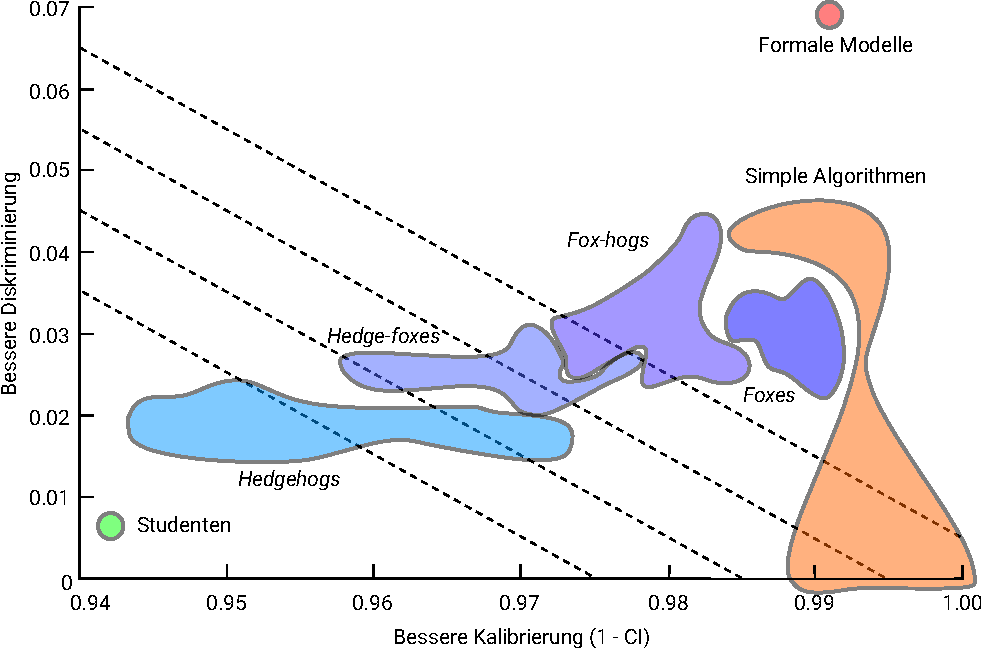
\includegraphics[scale=0.88]{Grafiken/Tetlock_2_Ink.pdf} 
\label{pic:Tetlock_2}
\end{figure}
Ein Ergebnis von Tetlocks \emph{forecasting exercises} wurde bereits in
Abbildung~\ref{pic:Tetlock_1} aus Teil~\ref{part:Schw_Vorhersagen} erläutert.
Dort war ersichtlich, dass die Experten im Vergleich zu statistischen
Algorithmen schlecht abschnitten. 

Abbildung~\ref{pic:Tetlock_2} zeigt nun ein differenzierteres Bild von der
Leistung der Experten\footnote{
Graphik basierend auf dem Original aus \cite{Tetlock} auf S.~77.
}. Abgebildet wird die Streuung der Leistung der Prognostiker in Abhängigkeit
von ihrem jeweiligen \emph{cognitive style}\footnote{
Wie in Abbildung~\ref{pic:Hedgehog_Fox} wird eine Unterscheidung zwischen
\emph{foxes}, \emph{fox-hogs}, \emph{hedge-foxes} und \emph{hedgehogs} gemacht.
}. Abbildung~\ref{pic:Tetlock_2} ist analog zu Abbildung~\ref{pic:Tetlock_1}.
Insbesondere sind wieder Kalibrierung und Diskriminierung\footnote{
Kalibrierung und Diskriminierung messen die Qualität der Vorhersagen eines
menschlichen Prognostikers oder eines (statistischen) Prognosemodells
(siehe S.~\ref{Kal_Dis}). Kalibrierung beschreibt die Fähigkeit eines
Prognostikers Ereignisse in richtige Wahrscheinlichkeitskategorien einzuordnen
(10\%-Ereignisse treten in 10~\% der Fälle ein, 20\%-Ereignisse in 20~\% der
Fälle usw.). Hohe Diskriminierung hingegen wird erreicht, wenn der Prognostiker
die Auftrittswahrscheinlichkeit einzelner Ereignisse von der Basisrate (
\emph{base rate}) aller Ereignisse unterscheiden kann. 
} in derselben Weise auf den Achsen abgebildet. Je weiter rechts-oben die
Wertung eines Prognostikers liegt, desto besser hat er bei den
\emph{forecasting exercises} abgeschnitten.

In Abbildung~\ref{pic:Tetlock_2} wird deutlich, dass die Urteilskraft der
Expertengruppen im Hinblick auf Kalibrierung und Diskriminierung variiert. Die
\emph{hedgehogs} erzielen die schlechtesten Wertungen unter den Experten,
während \emph{foxes} und \emph{fox-hogs} die besten Wertungen erhalten.
Insbesondere sind \emph{foxes} den \emph{hedgehogs} sowohl bezüglich der
Kalibrierungs- als auch bezüglich der Diskriminierungswertung überlegen.

Die statistischen Algorithmen waren allerdings besser als \emph{foxes} und
\emph{hedgehogs}. Die besten \emph{foxes} erhielten ähnliche Wertungen wie
Extrapolationsalgorithmen. \emph{Hedgehogs} machten hingegen so große Fehler,
dass ihre Wertungen in der Nähe des zufallsbasierten Algorithmus liegen
\footnote{
Tetlock gebraucht als Umschreibung für den zufallsbasierten Algorithmus die
Metapher des \glqq{Dart spielenden Schimpansen}\grqq
(\emph{dart-throwing chimp}).
}. Insgesamt konnte keiner der Experten, weder \emph{foxes} noch
\emph{hedgehogs} auch nur annähernd in die Nähe der Wertung kommen, die vom
autoregressiven Modell\footnote{
Als Stufe 3 Algorithmus in Abbildung~\ref{pic:Tetlock_1} und als formales
Modell in Abbildung~\ref{pic:Tetlock_2} bezeichnet.
} erreicht wurde. (vgl. \cite{Tetlock}, S.~118)

 
\subsection{Gründe für die schlechte Leistung der Experten}



Die in der Wissenschaft geschätzte Fähigkeit, mit wenigen Grundregeln oder
Axiomen auszukommen, scheint sich in eine Schwäche zu verwandeln, wenn
es darum geht, Prognosen für die reale Welt zu erstellen (vgl. \cite{Tetlock},
S.~68).

Insgesamt wird die Befürchtung, dass sich Menschen durch Wunschdenken leiten
lassen (vgl. \cite{Eisenfuehr}, S.~181) und dass sie das oft tun, von Tetlocks
Arbeit bestätigt.


%-------------------------------------------------------------------------------
Tetlock ist der Meinung, dass die Kernaufgabe politischer Weltanschauungen
nicht die Erstellung möglichst korrekter Prognosen ist, sondern die
Aufrechterhaltung einer bequemen Illusion von Berechenbarkeit
(vgl. \cite{Tetlock}, S.~39). Somit sind die Ergebnisse schlecht, weil keine
genaue Abbildung der Realität beabsichtigt wird. Die Aufrechterhaltung von
Glaubenssätzen, die zum kollektiven Zusammenhalt beitragen, hat höhere
Priorität.

In diesem Zusammenhang sind auch verschiedene Interpretationen des
Wahrheitsbegriffs bedeutsam. Eine weit verbreitete Interpretation wird mit
Hilfe des Pragmatismus von William James definiert. Demnach werden
Aussagen von Menschen als Wahrheit akzeptiert, falls die Aussagen ihnen bei der
Orientierung in der Welt nützlich sind. Dies liefert eine Erklärung dafür, dass
Menschen dazu tendieren Aussagen zu glauben, die ihre eigene Weltsicht
bestätigen. Bei einer extremen Ausprägung des pragmatischen Wahrheitsbegriffs
wird aus der Nützlichkeit einer Aussage ihr Wahrheitsgehalt abgeleitet:
\glqq{Es ist wahr, weil es nützlich ist}\grqq. (vgl. \cite{Precht})

Diese radikale Wahrheitsinterpretation ist problematisch, wenn die als Wahrheit
betrachteten Grundsätze der Realität widersprechen. Denn es gibt keine
Möglichkeit, die Grundsätze mit Hilfe von empirischen oder logischen Beweisen
zu revidieren und an die Realität anzupassen. Langfristig führen falsche
Grundsätze somit zu schlechtem Urteilsvermögen, was wiederum zu schlechten
Entscheidungen führt. Insbesondere sind Datenanalysen in einer solchen Situation
nicht zweckdienlich, da Ergebnisse selektiv ignoriert oder abgelehnt werden.

Eine andere Interpretation von Wahrheit legt großen Wert auf die Beweisbarkeit
von Aussagen. Eine solche Interpretation ist beispielsweise in der Wissenschaft
verbreitet. Aussagen wird erst dann ein Wahrheitswert zugewiesen, wenn
unwiderlegbare Beweise für die Gültigkeit der Aussage vorhanden sind. Eine
solche Interpretation weicht stark vom pragmatischen Standpunkt ab, kann aber
ebenfalls problematisch werden. Es besteht die Gefahr sich bei der Prüfung von
Aussagen in Kleinigkeiten zu verlieren, handlungsunfähig zu werden oder
nützliche Erkenntnisse zu lange anzuzweifeln\footnote{
Beispiele für Zweifel, die gefährlich werden, weil sie Fortschritt blockieren
sind auf Seite~\xcom erläutert.
}.

Vermutlich ist für ein gutes Urteilsvermögen ein nüchterner Pragmatismus
notwendig, bei dem vorsichtig zwischen Nutzen und Wahrheit abgewogen wird und
auch unangenehme Meinungen als Wahrheit akzeptiert werden können.
Bedauerlicherweise gerät ein solcher Pragmatismus mit jeder, insbesondere
politischen, Weltanschauung in Konflikt, die selbst nicht in dieser Art
pragmatisch ist.
%-------------------------------------------------------------------------------

\begin{table}
\centering
\caption{Ausgewählte Beispiele für kognitive Verzerrungen}
\label{tab:Kognitive_Verzerrungen}
\scalebox{0.7}{
\begin{tabular}{ |l|l|l|  }
\hline
\textbf{Bezeichnung der kognitiven Verzerrung} & \textbf{Sinngemäße Übersetzung}
  & \textbf{Kurzbeschreibung} \\
\hline
{ \large \emph{Anchoring} } & Ankereffekt
  & Beharren auf einer ersten \\
& & Schätzung eines Wertes; \\
& & unzureichende Anpassung\\
& & nach weiterem Überlegen.\\
\hline
{ \large \emph{Attribution bias} } & Zuschreibungsfehler
  & Die Tendenz, Erfolge \\
& & seinen eigenen Fähigkeiten \\
& & zuzuschreiben; \\
& & Misserfolge hingegen \\
& & externen Zuständen. \\
\hline
{ \large \emph{Availability bias} } & Verfügbarkeitsfehler
  & Beispiele für Szenarien, \\
& & die unmittelbar mit einem \\
& & Ereignis assoziiert werden, \\
& & bestimmen die Einschätzung \\
& & dieses Ereignisses. \\
\hline
{ \large \emph{Base rate neglect} } & Vernachlässigung von Basisraten
  & Vernachlässigung allgemeiner \\
& & Wahrscheinlichkeiten und \\
& & Konzentration auf fallspezifische \\
& & Informationen. \\
\hline
{ \large \emph{Cognitive conservatism} } & Kognitiver Konservatismus
  & Weigerung von Menschen, \\
& & Fehler zuzugeben und \\
& & ihre Meinung zu ändern. \\
\hline
{ \large \emph{Gambler's fallacy} } & Irrtum des Glücksspielers
  & Der irrtümliche Glaube an \\
& & regelmäßige Muster \\ 
& & in zufälligen Prozessen. \\
\hline
{ \large \emph{Hindsight bias} } & Rückschaufehler
  & Der Versuch eine Einschätzung \\
& & eines Ereignisses, nach dessen \\
& & Eintreten, rückwirkend zu \\
& & verändern. \\
\hline
{ \large \emph{Overconfidence effect} } & Selbstüberschätzung
  & Überschätzung der Richtigkeit \\
& & eigener Urteile. \\
\hline
\end{tabular}
}
\end{table}

\subsection{Auswirkungen von Tetlocks Forschungsergebnissen}

% TODO Zusammenfassung
% - Brier Score: große Zahlen -> Evidence
% - Bayes + einfache Statistische Regeln als Hilfswerkzeug
% - besser fox als hedgehog sein
% - Versuchen Kognitive Verzerrungen abzumildern
% - no thought above criticism (S. 118)
% - wenn möglich komplexere statistische Algorithmen verwenden

..., also \emph{predictive analytics} zu implementieren.

\section{Bestandteile von Predictive Analytics}

Bei \emph{predictive analytics} werden Daten mit Hilfe von geeigneten Methoden
verarbeitet, um verschiedene Arten von Prognosen zu ermöglichen. Dem
Datenanalysten stehen für diese Aufgabe Computeranwendungen zur Verfügung.
Diese Programme lesen die Daten ein, führen die notwendigen Berechnungen aus und
ermöglichen eine graphische Aufbereitung der Ergebnisse. \\ \\
Standardisierte
Vorgehensmodelle können helfen, die Arbeitsschritte einer Datenanalyse zu
vereinheitlichen. Ein Beispiel für ein solches Vorgehensmodell ist CRISP-DM
(\cite{crispdm}).

\subsection{CRISP-DM Vorgehensmodell}

(vgl. \cite{Runkler}, S.~3)

Zeigt eine beispielhafte Auswahl an Schritten, die in dieser Phase durchgeführt
werden können

\begin{table}
\centering
\caption{Vier Phasen Vorgehensmodell bei Datenanalysen}
\label{tab:Vier_Phasen}
%\scalebox{0.7}{
\begin{tabular}{ |l|l|  }
\hline
\textbf{Phase} & \textbf{Bestandteile} \\
\hline
Vorbereitung & Planung \\
  & Sammeln von Daten \\
  & Generierung abgeleiteter Attribute \\
  & Datenselektion \\
\hline
Vorverarbeitung & Daten aufräumen, \\
  & filtern, \\
  & ergänzen, \\
  & vervollständigen, \\
  & korrigieren, \\
  & standardisieren, \\
  & umwandeln \\
\hline
Analyse & Visualisierung \\
  & Korrelationsanalyse \\
  & Regression \\
  & Klassifikation \\
  & Clusteranalyse \\
\hline
Nachbearbeitung & Interpretation der Ergebnisse \\
  & Dokumentation \\
  & Evaluation \\
\hline
\end{tabular}
%}
\end{table}

\subsection{Daten}

\subsubsection{Elementare Datentypen}

Bei Daten lassen sich verschiedene elementare Typen\footnote{Alternativ dazu
spricht man vom Skalenniveau (\emph{scale of measurement}) als eine
Eigenschaft von Daten und Variablen.} unterscheiden.
Je nach Datentyp einer
Variablen, werden ihre Werte unterschiedlich interpretiert. Zudem können
bestimmte mathematische Operationen nur mit Variablen eines bestimmten Typs
durchgeführt werden. Die Datentypen werden im folgenden Text genauer erläutert
(vgl. \cite{Arens}, S.~1229 und \cite{McCarthy}, S.~28-29).\\ \\
Der \glqq{einfachste}\grqq Datentyp ist eine nominal skalierte Variable. 
Werte von nominal skalierten Variablen werden als Namen
interpretiert. Weiterhin ist es nicht sinnvoll diese Art von Variablen zu
ordnen. Es lässt sich lediglich feststellen, ob zwei Variablen
gleich oder ungleich sind. Ein Beispiel für eine nominal skalierte Variable ist
der Name einer Stadt. Die Werte sind dann konkrete Städtenamen wie
\glqq{München}\grqq oder \glqq{Berlin}\grqq. Als Operationen stehen nur $=$
oder $\neq$ zur Verfügung, weil Aussagen wie 
\glqq{München}\grqq$=$\glqq{München}\grqq oder
\glqq{München}\grqq$\neq$\glqq{Berlin}\grqq sinnvoll sind. Nicht sinnvoll wären
dagegen Vergleiche wie \glqq{München}\grqq$<$\glqq{Berlin}\grqq
\footnote{Der Vergleich wäre sinnvoll, wenn mit der Nennung des Namens 
z. B. implizit die Größe der Stadt gemeint wäre. Dies ist hier aber nicht der
Fall.}.
Weitere Beispiele für nominal skalierte Variablen sind Geschlecht, Augenfarbe
oder Postleitzahl. \\ \\
Etwas mehr Möglichkeiten stehen zur Verfügung, wenn eine ordinal skalierte
Variable vorliegt. Für eine solche Variable ist eine Ordnung sinnvoll, sodass
alle Vergleichsoperationen möglich sind. Eine Kleidungsgröße (\texttt{S},
\texttt{M}, \texttt{L}) ist ein Beispiel für eine ordinal skalierte
Variable. Im Gegensatz zum Beispiel mit den Städtenamen ist ein Vergleich wie
\texttt{S} $<$ \texttt{M} hier sinnvoll. \\ \\
Wird eine Variable auf einer Intervallskala definiert, sind ihre Werte
numerisch.
Zusätzlich zu
allen Operationen von nominal und ordinal skalierten Variablen können hier auch
Additionen und Subtraktionen ausgeführt werden. Ein Beispiel hierfür sind
Temperaturen in \degree{C}, die addiert und subtrahiert werden können.
Allerdings sind 20~\degree{C} nicht das Doppelte von 10~\degree{C}. Hier kann
man erkennen, dass es bei Intervallskalen nicht sinnvoll ist, Verhältnisse zu
berechnen. Der Grund hierfür ist, dass der Nullpunkt einer Intervallskala nicht
mit dem absoluten Nullpunkt einer Größe identisch sein muss. So sind
0~\degree{C} nicht der absolute Nullpunkt für die Temperatur. Wenn man sinnvolle
Verhältnisse berechnen will, wird eine Proportionalskala benötigt. \\ \\
Eine auf einer Proportionalskala definierte Variable hat numerische Werte, für
die alle zuvor erwähnten mathematischen Operationen definiert sind und
zusätzlich auch Multiplikation und Division möglich sind.
%Insbesondere ist es sinnvoll Verhältnisse zu berechnen.
So führt eine
Multiplikation einer Länge in Metern mit der Konstante 2 zu der doppelten Länge.
Ist das Verhältnis zweier Längen gleich 10, so ist die eine Länge 10
mal so groß wie die andere. Weiterhin führt die Multiplikation zweier Längen
in m zu einer korrekten Fläche in $\textrm{m}^2$. Die Ergebnisse wären nicht
korrekt, wenn der Nullpunkt der Meterskala nicht mit dem Nullpunkt der
Längenskala identisch wäre, wie es bei Intervallskalen der Fall ist. \\ \\
Nominal und ordinal skalierte Variablen sind qualitative Variablen.
Variablen, die auf Intervall- oder Proportionalskalen definiert sind, werden
hingegen als quantitative oder kardinale Variablen bezeichnet.
Weiterhin werden qualitative Variablen auch als kategorisch
(\emph{categorical}) bezeichnet, quantitative als numerisch (\emph{numeric})
und je nach Wertebereich als diskret (\emph{discrete}, ganzzahlige Werte) oder
kontinuierlich (\emph{continuous}, Fließkommawerte). \\ \\
Tabelle~\ref{tab:Skalen} zeigt eine Zusammenfassung der verschiedenen Datentypen
und der erlaubten Operationen\footnote{
Basierend auf Tabelle 2.2 in \cite{Runkler}, S.~8}.
\begin{table}
%\footnotesize
\centering
\caption{Übersicht der Datenskalen}
\label{tab:Skalen}
\scalebox{0.7}{
\begin{tabular}{ |l|l|l|l|  }
\hline
\textbf{Skala} & \textbf{Sinnvolle Operationen}
  & \textbf{Beispielgrößen} & \textbf{Beispielwerte} \\
\hline
Nominal & Gleichheit ($=, \neq$) & Name, & \glqq{Julia}\grqq,
  \glqq{Klaus}\grqq \\
& & Geschlecht & \texttt{M}, \texttt{W} \\
\hline
Ordinal & Gleichheit ($=, \neq$), & Kleidungsgröße & \texttt{S}, \texttt{M},
  \texttt{L} \\
        & Vergleiche ($<, >, \ldots$) & & \\
\hline
Intervall & Gleichheit ($=, \neq$), & Jahresangabe, & 2015~n.Chr. \\
  & Vergleiche ($<, >, \ldots$), & Temperatur in Grad Celsius & 20~\degree{C} \\
  & Addition ($+$), Subtraktion ($-$), &  &  \\
\hline
Proportional & Gleichheit ($=, \neq$), & Alter, & 21 Jahre \\
  & Vergleiche ($<, >, \ldots$), & Temperatur in Kelvin & 273.4~K \\
  & Addition ($+$), Subtraktion ($-$), &  &  \\
  & Multiplikation ($\cdot$), Division ($/$) & & \\
\hline
\end{tabular}
}
\end{table}


\subsubsection{Information Management (Data Warehouse)}

\subsubsection{Datenabhängige Ziele}

\paragraph{\ldots}

\paragraph{Beschreibung der Daten}

\paragraph{Klassifikation}

\paragraph{Zeitreihenanalyse}

\subsection{Methoden}

\begin{figure}%[!hbt]
\centering
\caption{\emph{Predictive analytics} Methoden aus der Anwenderperspektive.}
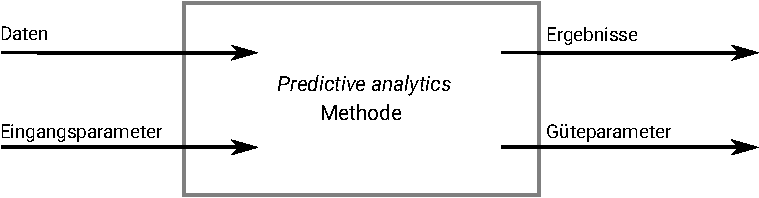
\includegraphics[scale=1.0]{Grafiken/PA_Methoden_Ink.pdf} 
\label{pic:PA_Methoden}
\end{figure}

\subsubsection{Die Großen Drei}

\paragraph{Regression}

\paragraph{Entscheidungsbäume}

\paragraph{Neuronale Netze}

\subsubsection{Zeitreihenanalyse}

\subsubsection{\ldots}

\subsection{Werkzeuge}

\subsection{(Kreative) Freiheitsgrade bei der Implementierung eines
  Vorhersagemodells}

\section{Anwendungsbeispiele}

\subsection{Allgemeine Anwendungsfelder (siehe SAP Artikel)}

\subsection{\ldots}

\section{Allgemeine Risiken bei der Nutzung von Predictive Analytics}

Es existieren Risiken, die dazu führen können, dass die Ziele einer
Datenanalyse nicht oder nicht in vollem Umfang erreicht werden können.
Im folgenden Text werden einige dieser Risiken erläutert.

\subsection{Risiko der Unverhältnismäßigkeit}

Die Anwendung von Predictive Analytics ist mit einem hohen Aufwand verbunden.
Dabei spielen die Kosten für die Datenerhebung eine wesentliche Rolle.
Zusätzlich werden für die Datenanalyse Kenntnisse aus verschiedenen
Fachrichtungen benötigt. So sind einerseits anwendungsspezifische Kenntnisse
zur Interpretation der Daten und der Ergebnisse wünschenswert. Andererseits
werden zur Durchführung der Datenanalyse Kenntnisse in Mathematik, Statistik und
Informatik benötigt. \\ \\
Aus diesem Grund besteht das Risiko, dass die Kosten einer Anwendung von
Predictive Analytics den Nutzen übersteigen. Es ist auch möglich, dass das
gleiche Ergebnis mit einer einfacheren, kostengünstigeren Methode erreicht
werden kann. In diesem Fall würde die Anwendung eines aufwändigen Predictive
Analytics Verfahrens wertvolle Ressourcen binden, die an anderer Stelle stärker
gebraucht werden. \\ \\
Somit ist es wichtig, Betrachtungen zu Alternativkosten \todo{gls eintrag}
in die Planung von \emph{predictive analytics} Anwendungen einzubeziehen. 

\subsection{Risiken bei der Datenerhebung}

Trainingsdaten spiegeln nicht (mehr) das Verhalten des Systems wider.

\subsubsection{\ldots}

\subsection{Risiken bei der Interpretation der Daten}

\subsection{Risiken bei der Interpretation der Ergebnisse}

Wenn die Ergebnisse der Datenanalyse zur Entscheidungsunterstützung herangezogen
werden, beeinflussen sie das Verhalten der Entscheidungsträger. Dies kann zur
Entstehung problematischer psychosozialer Effekte führen. Zwei Beispiele hierfür
werden nun erläutert.

\subsubsection{Prognose verändert das Verhalten des Systems }

Die Ergebnisse von Vorhersagen werden von Menschen interpretiert,
die daraufhin ihr Verhalten anpassen. Dies kann zu Rückkopplungseffekten führen,
die von negativen Auswirkungen im Sinne einer
\glqq{Selffulfilling} Prophecy\grqq begleitet werden können
(vgl. \cite{Crossman}). Bestimmte Prognosen können beispielsweise von einer 
Interessengruppe als Bestätigung ihrer Agenda interpretiert werden, wobei
anders lautende Vorhersagen ignoriert werden. Dadurch bestärkt, setzt die Gruppe
ihre gewünschten Handlungsoptionen um. Dies ruft den vorhergesagten Effekt
jedoch erst hervor.

\subsubsection{Ignorieren der Unsicherheiten bei der Prognose}

Es besteht die Gefahr, dass die Unsicherheiten von Vorhersagen ignoriert werden
und die Prognose als eine Gewissheit betrachtet wird. Somit wird möglichen,
alternativen Entwicklungen bei der Entscheidungsfindung nicht genügend Bedeutung
beigemessen. Dies kann dazu führen, dass Risiken falsch kalkuliert werden und
in der Zukunft nicht genügend Handlungsoptionen zur Verfügung stehen.
